% Chapter 4
\chapter{Advertisement decision} % Main chapter title

\label{Chapter4} % For referencing the chapter elsewhere, use \ref{Chapter1} 
\newpage



\section{Introduction}
At the time of industrialization, industries compete on product quality, and modern organizations focused more on delivering services, and now services and products is hardly able to be distinguished because of they provide various offers and consumers lose themselves in it, as Peter van Waart describes in his paper that ``\emph{In the last two decades however, economical developments resulted in the experience economy: a new era of marketing and branding, in which traditional advertising is becoming less effective and meaningful experience branding is key}'', \cite{Meaningful_ad}, therefor economical developments have changed from time to time and is emerging from economical experience and factors like price-reduction for a brand is not so important, but experience factor has become the central part for the development.Any advertisement that explains a product features and why that matters fails to achieve people satisfaction, because people’s experience were not considered in it, as Joško Brakus \cite{Brand_experience} explains the measurement of brand experience and how it can effect on product loyalty.

Now at this era where the technology is highly advanced and most people especially youngsters are much familiar with them like using smartphones, tablets and now even wearable computers like Apple watch, and also there are many developments in sensing technologies like body tracking, hand recognition, by using these technologies different interactions are possible and very attractive and funny interactive advertisement can be developed so that could engage more participants.

The development of advertisement requires many steps and the initial step is to create content and this happens normally by creating a \emph{Focus group} of stakeholders or producers to be able to fully convey their message through advertisement. Focus group is a small group, usually between six up to ten participants, that joint together in comfortable place, usually a quite room, to discuss on a specific topic domain and share ideas. As described by Jenny Cameron ``\emph{Focus groups can be exhilarating and exciting, with people responding to the ideas and viewpoints expressed by others, and introducing you, the researcher, and other group members to new ways of thinking about an issue or topic }''\cite{FocusGroup}.As Florian Alt \cite{mobile_focus_group} talks about the process of how the focus group was conducted for a mobile contextual display systems.

As a computer scientist, there had been no chance to create an advertisement, and this was the opportunity to make one, and after negotiating with University communication department and then discussing with University marketing department, finally the decision was made to make an advertisement for \emph{Bauhaus-Walk}\footnote{Bauhaus Walk: https://www.uni-weimar.de/en/university/profile/bauhausatelier/bauhaus-walk/, last accessed 26 may 2016}, which was conducting tours about Bauhaus for tourists in Weimar, but in-depth goal and motivation of this program was not clear, what kind of advertisement they wanted, what message they wanted to convey through the advertisement was not clear.    

Therefor, there was a need to conduct a focus group to do requirement analysis on \emph{Bauhaus-Walk} program and its content. This was mainly meant to understand many aspects of Bauhaus-Walk and collect the required parameters for designing the advertisement (interactive and non-interactive). Because of time limitation in each session two sessions were arranged in two different dates to cover all topics and discussions. This chapter describes the main theme and goal for focus group and reports all the processes that were taken to establish the focus group, how participants were invited and what was being discussed and more focused on each session. How data was gathered and what techniques were used to analyze them. The document presents all the findings and outcomes in details and related discussions and conclusions.



\section{Research Questions}
To design and create the Bauhaus-Walk advertisement, it was required to collect the below information from the Bauhaus-Walk members, so that a very relevant and meaningful advertisement could be developed that could speak by itself for Bauhaus-Walk and at the same time it should be entertaining and funny and fit for both interactive and non-interactive advertisement, so that passers-by remember the experience for long time and as a result be motivated to take the tour. Therefor we would need to understand many aspect of Bauhaus-walk as listed below in short.

\begin{enumerate}
\item Who is (are) the target group?
\item What are the existing Bauhaus-Walk advertisement medium?
\item What are the peak times in the year and famous locations for Bauhaus-walk tour?
\item What are important aspects of Bauhaus-Walk from their point of view?
\item What could be a suitable advertisement theme and content?
\item What interactions should be integrated in interactive (body \& Mobile) advertisement?
\end{enumerate}


\section{Study design}
Focus group was designed in two sessions mainly because the participants could not be present all at the same time or date, and by doing this, there was enough time to analyze the first session and discuss the findings in the second session with new participants and get their point of views, the first session was more related to gathering general information about Bauhaus-Walk program and second session was more in depth discussions on the advertisement decisions.

\subsection{Participants and Environment}
The focus group in the first session consisted of three participants, and in the second session it consisted of two participants. The participants of this focus group were only active tour guides for Bauhaus-Walk, they have been providing tours for more than a year and know the aim and vision of Bauhaus-Walk, They were invited through Doodle\footnote{Doodle: http://doodle.com/de/, last accessed: 26 May 2016}, where varieties of date slots were available to select, in which a short introduction of the aim of the focus group was also described to. Both sessions lasted for 90 minutes.

\begin{figure}[H]
    \centering
    \begin{subfigure}[H]{0.45\textwidth}
        \centering
        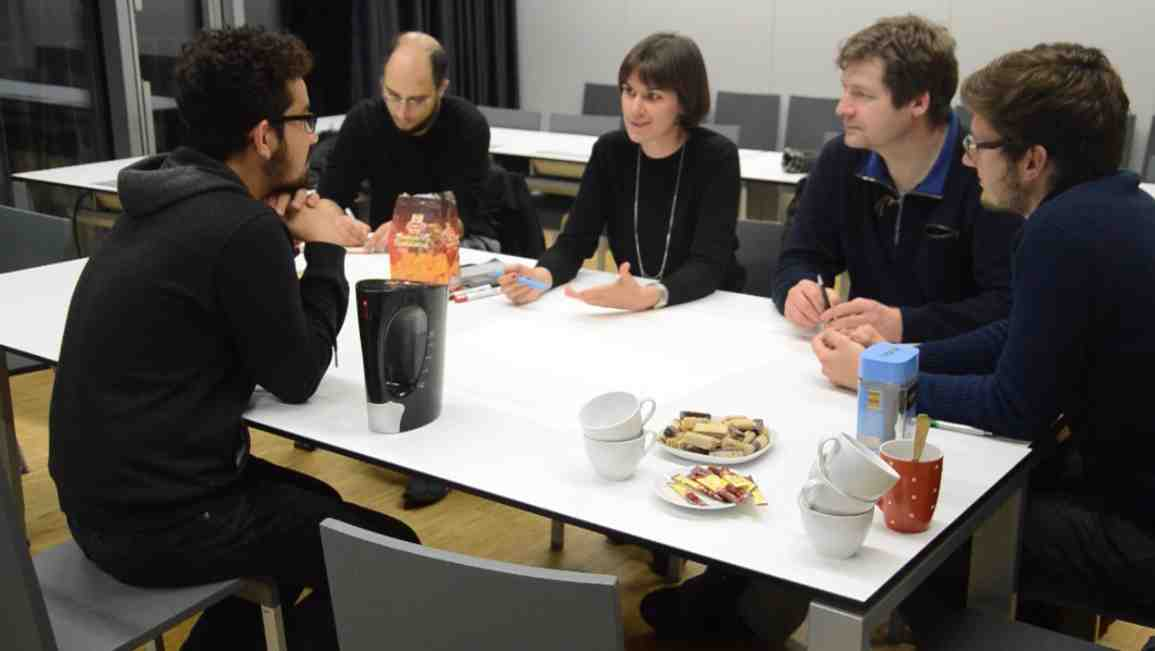
\includegraphics[width=\textwidth,height=4cm]{Figures/4/focus_group_s1}
        \caption{1st Session focus group }
        \label{fig:focus_group_s1}
    \end{subfigure}
    \begin{subfigure}[H]{0.45\textwidth}
        \centering
        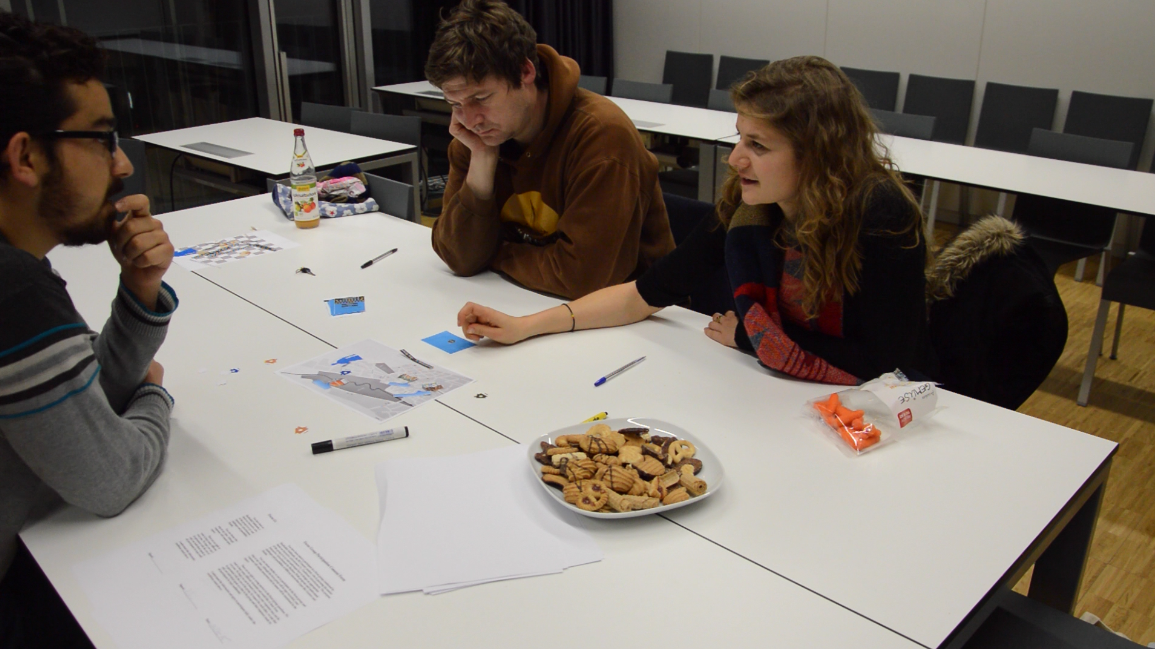
\includegraphics[width=\textwidth,height=4cm]{Figures/4/focus_group_s2}
        \caption{2nd Session focus group}
        \label{fig:focus_group_s2}
    \end{subfigure}
    \caption{Focus group sessions}
    \label{fig:Focus_group_sessions}
\end{figure}

The focus Group was held inside the DBL\footnote{DBL: Digital Bauhaus Lab} building in meeting room, where we had enough space to make a group circle. Participants were offered coffee and biscuits at the beginning or end of the session to feel comfortable and relaxed for discussion.


\subsection{First session}
This session was an exploratory session over Bauhaus-Walk program, and it was a good start for me to investigate thoroughly on related program domains to create the prototypes for the next sessions.


\subsubsection{Procedures}
Participants were warmly welcomed and asked to feel comfortable by having biscuits and coffee. I introduced myself and asked them to introduce themselves. This helped to understand each others professional background and interests. 

\begin{enumerate}
\item Introduction \\
Brief introduction on advertisement and interactive advertisements were given to participants to understand the possibilities of existing technologies and the use of them in advertisement field. Some interactive advertisements were introduced with their relative interaction techniques. The agenda and goal of thesis was also described to have a wide picture of what is going to be done till the end of this semester.

\item Consent Form \\
Each participant was asked to sign the consent form to make sure they agree to participate and video recorded.

\item Discussion session \\
After introduction, discussion started on below mentioned questions. Because there was limited number of participants I could not divide them in to groups to discuss in detail and do comparative study among the groups. They were given sheet empty big papers to draw and write what come in their mind while discussing to be able to keep track of their thoughts and be easy to generalize the opinions. During the discussion Patrick Tobias Fischer was asked to write notes on the discussion.

\begin{enumerate}
\item   What kinds of advertisements for Bauhaus-Walk are there?
\item   Who join the Bauhaus-Walk program in general?
\item   What could be a suitable theme of Bauhaus-Walk for the Interactive advertisement?
\item   What would be the content of the advertisement?
\item   How to motivate passer-by to be engaged with the advertisement?
\item   How to engage passers-by with the advertisement?
\item   What kind of Gesture and Mobile Interactions should be used?
\item   How to motivate passer-by to join the actual Bauhaus-Walk tour?
\item   Is there anything else we need to discuss on Bauhaus-Walk Advertisement? Any new angle?

\end{enumerate}


\end{enumerate}


I was responsible to carry on the entire discussion and Patrick Tobias Fischer was doing the note taking during the discussion. He noted important information extracted from our discussions so that I could later look at them beside that, the entire discussion was also video recorded for analyzing.



\begin{figure}[H]
    \centering
    \begin{subfigure}[H]{0.45\textwidth}
        \centering
        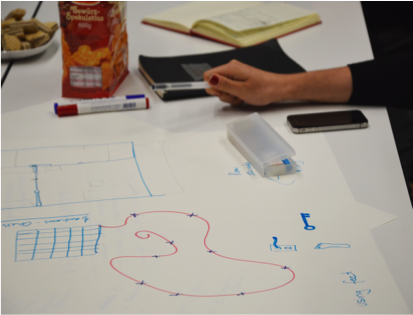
\includegraphics[width=\textwidth,height=5cm]{Figures/4/drawings}
        \caption{Drawing sketches}
        \label{fig:focus_group}
    \end{subfigure}
    \begin{subfigure}[H]{0.45\textwidth}
        \centering
        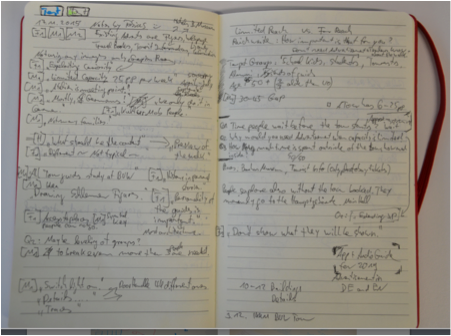
\includegraphics[width=\textwidth,height=5cm]{Figures/4/notes}
        \caption{Observation notes}
        \label{fig:meeting_room}
    \end{subfigure}
    \caption{Discussion Session}
    \label{fig:observation_env_observation_note}
\end{figure}


\subsection{Second Session}
Based on the first focus group's discussions and the participant's nice ideas, which are mentioned in finding section, two different paper prototypes of advertisement were made to dig more in detail. The participants were given the prototypes to play with them and explore their own way of designing the advertisement and interaction.

The basic ideas were designed to help the participants to think more and come up with some more ideas and at the same time should be in the context of Bauhaus-Walk program. 

\subsubsection{Procedures}
\begin{enumerate}
\item   Short introduction was given on Interactive Advertisement thesis.
\item   Consent forms were handed to sign for video recording.
\item	Short motivational video of interactive advertisement was shown.
\item	Two paper prototypes that are mentioned above (Bauhaus chess and Map) were introduced.
\item	Possible interactions were shown to them.
\item	Participants were asked to comment on prototypes and come up with new ideas and interactions.
\item	They were asked to design their own prototype.
\item	Integrate some fun ideas with prototypes.
\item	What contents should be included in the prototypes.
\item	How to gather and collect those contents.
\end{enumerate}

\subsubsection{Prototypes and discussion}
Two prototypes were explained to the participants, that how the prototype originated from the previous discussions, how the prototype functions, a short glance to these prototype are described below. 

First prototype was Bauhaus-Chess, This prototype was chosen because of the historical background of this amazing chess game that was developed by Josef Hartwig\footnote{Josef Hartwig: http://bauhaus-online.de/en/atlas/personen/josef-hartwig, last accessed: 26 May 2016} long time before. The shape of the chess piece defines the movement direction of itself on the chessboard. The goal was to show the chess on the advertisement screen and show one piece at a moment and let users to move the chess in the right direction by some sort of gesture. 

Second prototype was to show a city map on the screen with possible interactive famous places of Bauhaus, the interaction idea was to map physical movement of a person or map the cursor movement of a phone to the virtual movement on the city map, and let user to explore the target places by reaching to those locations. Maximum three places were to be explored by one person to finish the interaction.


\begin{figure}[H]
    \centering
    \begin{subfigure}[H]{0.7\textwidth}
        \centering
        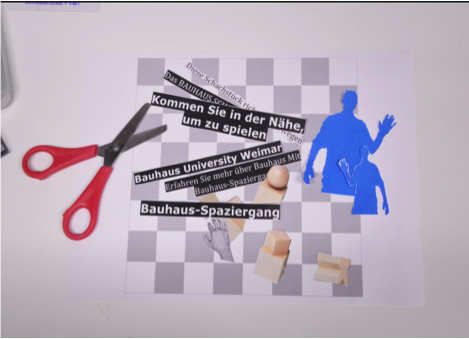
\includegraphics[width=\textwidth,height=6.5cm]{Figures/4/chess}
        \caption{Chess prototype }
        \label{fig:chesspro}
    \end{subfigure}
    \begin{subfigure}[H]{0.7\textwidth}
        \centering
        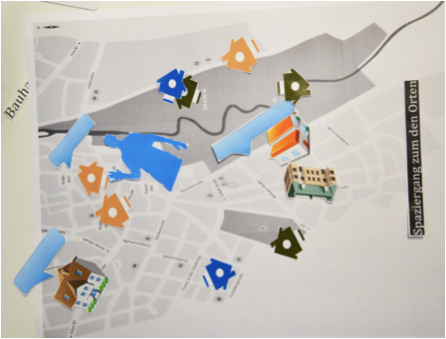
\includegraphics[width=\textwidth,height=6.5cm]{Figures/4/map}
        \caption{Map prototype}
        \label{fig:mapprot}
    \end{subfigure}
    \caption{Prototypes}
    \label{fig:map_chess_prototypes}
\end{figure}


After prototype got explained to the participants, they were asked to bring their own ideas and ask questions, find possible issues and how to enhance one of them to be used for the advertisement. The consideration was also that any prototype selected should be valid for non-interactive, body interactive and mobile interactive advertisement.


\begin{figure}[H]
    \centering
    \begin{subfigure}[H]{0.45\textwidth}
        \centering
        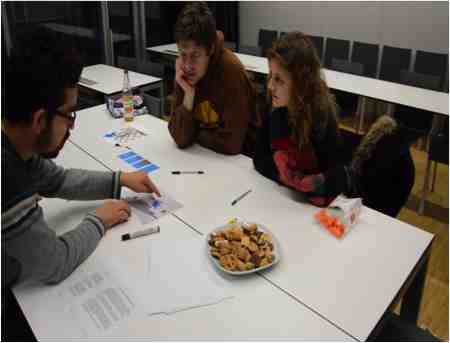
\includegraphics[width=\textwidth,height=5cm]{Figures/4/show_map}
        \caption{}
        \label{fig:showmap}
    \end{subfigure}
    \begin{subfigure}[H]{0.45\textwidth}
        \centering
        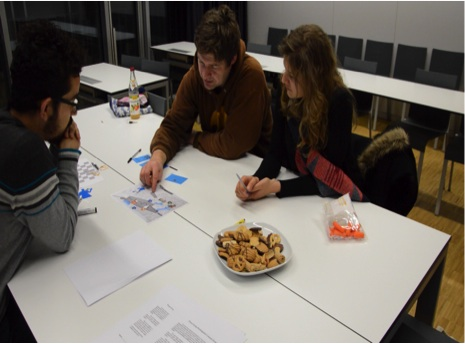
\includegraphics[width=\textwidth,height=5cm]{Figures/4/tell_map}
        \caption{}
        \label{fig:tell_map}
    \end{subfigure}
    \caption{Explaining and discussions on prototypes }
    \label{fig:explaining_and_discussion}
\end{figure}

\subsection{Data Gathering}
The data gathering design of the focus groups were done in a way that could be very easy to be analyzed and generalized in very little amount of time. 


\begin {itemize}
\item   The participants were encouraged to discuss the issues on a piece of chart using drawings and texts this helped the participants to focus on their ideas and build the ideas in a more better way and at the same time that helped the research to have a summary of their opinions and thoughts 
\item   They could make summary of their discussion on the paper so that they and I fully understand the topics. see Appendix (\ref{app:Sk1}, \ref{app:Sk2} and \ref{app:Sk3}) for sketches.
\item   Tobias Patrick was taking notes to cover up everything we discussed.
\item   All the sessions were video recorded for full detailed analyzing. 
\item Photos were also taken from the participant while discussing ideas, and also from the sketches they drew.
\end{itemize}


All of the above resources were analyzed by going through each of the sketches they drew and each notes that were written and all the videos were seen many times to check if some ideas were not clear in the sketches or notes and to have a final image of the discussions.


\newpage
\section{Findings}

\subsection {First Session Findings}
The below sections are extracted from the long discussions, and analyzing video and drawn charts.


\subsubsection{Bauhaus-Walk}
\emph{Bauhaus-Walk} is a project that is run by university students to show more about Weimar and Bauhaus culture to the world, by giving small tours to group of maximum 30 people. The tour shows studying conditions of the university and students, living style of people and giving excursion to historical places.

Tour guides are from different backgrounds like architecture, urbanism and design and each of them could show various aspect of Bauhaus by their own stories, and interrelate the stories with the facts and then connect them to the places in Weimar. Most important for the guides are not just the buildings, but also the small details inside the building that most people do not focus. The guides want to be the voice of those unspoken stories for the tourists.

\subsubsection{Current Advertisements}
Current existing advertisements for Bauhaus Walk is through different mean as listed below.

\begin {enumerate}

\item	Web: \\
Bauhaus Walk is advertised briefly in the Bauhaus University Weimar webpage\footnote{Bauhaus Walk: \url{ https://www.uni-weimar.de/en/university/profile/bauhausatelier/bauhaus-walk/}} and in Weimar tourist information page\footnote{Weimar tourist information: \url{http://www.weimar.de/homepage/}, Last accessed, 4th Jan 2016}.

\item	Print: \\
Bauhaus Walk program are advertised in flyers and leaflets at different locations, like they could be found in tourist information center, Bauhaus Museum, calendar of Weimar and in travel leaflets. 

\item	Books: \\
Bauhaus Encyclopedia has mentioned this program too. 

\item	Oral: \\
Mostly the people who have already taken the program once publicize it and they let their friends, relatives and family know about it.
\end{enumerate}


\subsubsection{Tour participants}
Most of the people who join the tour are from elder people range between 45-65 years old and others are adults and children. Adults mostly learn about the program trough web and the elders learn from the tourist information centers and books.  Most of the participants are German and do not understand English language.

\begin{figure}[H]
    \centering
    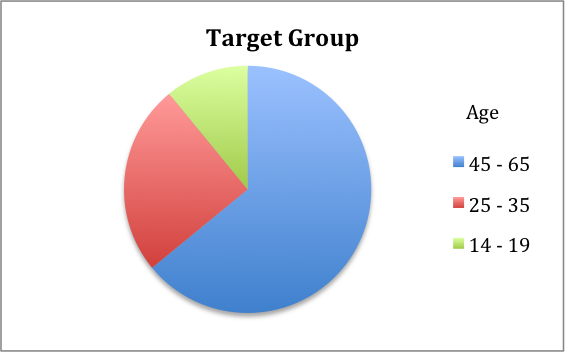
\includegraphics[width=8cm, height=5cm]{Figures/4/target_group}%
    \caption{Tour participant average ages}%
    \label{fig:target_group}%
\end{figure}


\subsubsection{Peak Tour times}
In Average 5000 people take the tour each year. April, May, September and October are the peak months that people take the tour because of the weather condition to be good the amount of people per tour is about 25 people, but in winter there are very few people joining the tour and the amount of people per tour is up to five to six. 

\subsubsection{Possible advertisement location}

\begin {enumerate}

\item	Tourist Information. \\
This is a good place to put Bauhaus-Walk advertisement because 
\begin {itemize}
\item	Random visitors from different places and cities come here and want to know about Weimar in general. 
\item	Heavy traffic of people.
\item	This is the only place to get Bauhaus-Walk tickets in advance.
\end{itemize}


\item	Bauhaus Museum. \\
This could be another good place, but people have to pay to enter to this museum, so there will be limited people but who
\begin {itemize}
\item	Are very interested in Bauhaus.
\item	Likely to go on tours.
\end{itemize}


\item	University main building. \\
Main university building is a more open place for all visitors; there are many factors as stated below.

\begin {itemize}
\item	People from different background.	
\item	People from different age, more youngsters like students.
\item	Interested people in Bauhaus.
\item	It is close to starting point of Bauhaus-Walk tour.
\end{itemize}


\end{enumerate}


\subsubsection{Content of advertisement}
Participants pointed on very important things about the content of advertisement, from which the advertisement got clearer and clearer and could be categorized in to many different aspects of Bauhaus-Walk.


\begin {enumerate}

\item	Objects \\
There are objects that are introduced during the tour for the tourists; A good idea would be to show those objects on various locations on the map that belong to.
\item	Stories \\
Bauhaus Walk tour guides have many stories to tell about the walk and their own backgrounds as one of them said ``\emph{Probably our walk is to sum it up, consists of stories we are actually telling stories, not just talking about history, not just about facts but our own personal stories and stories that were told by former students, so we are kind of raping the history in to personal stories, and we want to say that hay, we are students from different faculties and we want to tell the stories by different ways, and that is not a bad thing, because based on historical fact that there has not been the same Bauhaus in Weimar, there has been so many different teachers and students and they all had a different idea that what Bauhaus could be and I think we still kind of incorporate that the fact that no Bauhaus tour would be the exactly the same like the others before.}''
\item	Histories, Facts, Places \\
The content of advertisement could also be related to history of Bauhaus, how it is known to world, what were and are the innovations and obviously show the historical buildings of Bauhaus.


\end{enumerate}

\subsubsection{Interaction of advertisement}
Based on the examples that were shown at the introduction for the participants, they liked hand gesture and some other techniques and came to the below possible techniques.

\begin {enumerate}
\item	Hand gesture Interaction. \\
The below two kinds of interactions were discussed each containing different contents. 

\begin {itemize}
\item	Hovering: \\
By showing the Bauhaus map on the screen with the most important elements on it, the users should be able to look at the items by moving their hands on top of it. The items could change its status when hovering for example if there is a light object shown by hovering it should turn on or something like that.
There could be famous places shown on the map that Bauhaus-Walk tour focuses most, and by hovering the hand some more information like a picture or a related to that places should be shown.

\item	Performing a specific gesture:\\
There are many objects that have specific characteristics and those details are described in the tour, so the idea was to bring those objects in action and allow users to perform those actions, one idea was to show a 3D environment and the user should be able to perform a gesture, like opening door handle, lighting up a lamp, opening a lock by a key or play with Bauhaus \emph{Bauhaus- Schachspiel}\footnote{Bauhaus-Schachspiel: \url{http://www.markanto.de/Markanto-Store/Entwurfsjahr/1920-1929/Bauhaus-Schachspiel::165.html},last accessed: 27 May 2016 }(chessboard) to navigate the correct movement of the chess piece on to the screen, or other different gestures for specific tasks.
\end{itemize}

\item	Body Interaction  \\
Bauhaus-Walk is known from its name that it is all about walking to different historical places, therefor there was the idea of giving short virtual walk on the screen by moving the user's body in front of the screen and exploring some sights.

\end{enumerate}


\subsection{Second Session Findings}
The second session was held after a week and half, with only two participants other participants could not come because they were busy with their studies. 

\subsubsection{Prototype discussion}
After lengthy discussion on both prototypes, that how could they fit for both mobile and body interactions and at the same time for non-interactive advertisement and whether or not these prototypes could be ideal for Bauhaus-Walk theme and could convey their message through it or not. The below are their final summarized comments on both prototypes. 

\begin {enumerate}

\item Chess-Game

\begin {itemize}

\item{Positive points:} 

\begin {itemize}
\item	The idea is very nice, because many of the visitors are above the age of 40 and they may be familiar with this game.
\item	Easily understandable by looking at the shape, because shape defines the movement. 
\item	Suites best for Bauhaus Museum because, there is the original chess board of Bauhaus but people are not allowed to touch the game, by bringing this type of interaction, people will have a live experience with the chess board and play around with it and understand it.

\end {itemize}

\item{Negative points:} \
\begin {itemize}
\item	Very difficult to understand by people who have not played chess before or have not seen this special type of chess.
\item	Players could make a lot of mistakes while moving the chess piece. 
\item	The idea does not really fit to the Bauhaus-Walk program.
\item	It does not fit the places that are being shown in the tour.
\end {itemize}
\end {itemize}

\item Map-Game 

\begin {itemize}

\item{Positive points:} 
\begin {itemize}

\item	Map game idea fits a lot to Bauhaus-Walk tour.
\item	Portraits the idea of walking action.
\item	Easy interaction just by moving body or a cursor in mobile phone and navigate inside the screen.
\item	Understandable concept by moving on to different places and exploring them. 
\end {itemize}

\item{Negative points}
\begin {itemize}
\item Possible moving difficulties in a given space.
\end {itemize}
\end {itemize}
\end {enumerate}

\newpage
\section{Conclusion}
The conduct of the two sessions of focus group was very helpful in a way that it was held very intensive that helped to understand in general the whole about Bauhaus-Walk program tour and especially about the tour guides that what they think about Bauhaus-Walk and what are the most important things that could be discussed and advertised for Bauhaus-Walk. All the relevant mentioned questions for the design and interaction of advertisement were answered and discussed. As a result of this focus group, one interactive advertisement prototype would be purposed, that should be able to cover all the aspects of advertisement and concept of Bauhaus-Walk that was discussed in this focus group.

Based on the opinions and discussions, participants chose the Map-Game prototype to be developed for Bauhaus-Walk advertisement and this prototype would suite better in Tourist Information center than Chess-Game prototype. Along with the prototype decision, participants suggested more features were to be integrated with prototypes, like (1) Content of the game should be very clear and accurate and they should show the places where we provide tour. We do not have many places to show and there may be maximum three places.(2) Integrating some fun factor to the game and interaction like by showing a famous character face on top of the silhouette head position. And giving a kind of funny movement. (3) Giving opportunity for multiusers to play interactive game, like for example if there are two people standing in front of the screen, the tasks will be divided among them by locking one's silhouette or interaction and allowing the other to perform the task. (4) Defining the task by the defined character or by color of the body or by random. (5) Showing funny map, which was made many years back of Weimar city. (6)Popping up interactive objects (houses) on the screen so the users understand that they are interactive. 




